\chapter[Materiais e Métodos]{Materiais e Métodos}

\section{Hardware}

O desenvolvimento e as análises deste trabalho foram realizados em um computador Desktop com 500GB de espaço em disco, 4GB de RAM e 2 processadores Intel Pentium(R) Dual-Core E5400 @ 2.70GHz. Para o ambiente de produção foi utilizado um servidor Dell PowerEdge T-710 com 12TB de espaço em disco, 115GB de RAM e 24 cores Intel(R) Xeon(R) CPU X5660 @ 2.80GHz.

O pipeline de análise de exomas desenvolvido por este trabalho foi executado tanto no servidor local quanto no supercomputador do Centro Nacional de Processamento de Alto Desempenho de Minas Gerais (CENAPAD-MG) que possui 107 nós de computadores interligados através de uma rede rápida Infiniband com 8GB de RAM e 8 núcleos (Intel(R) Xeon(R) E5335 @ 2.00GHz) por máquina, totalizando 856 núcleos e 856GB de RAM disponíveis para serem utilizados para a execução de processos.

\section{Sistema Operacional}

O sistema operacional escolhido para o desenvolvimento deste projeto foi o Biolinux \cite{Field2006} atualmente na versão 8.0. Este é um sistema baseado em Ubuntu que foi criado e mantido pelo ``NERC Environmental Bioinformatics Centre'' na Inglaterra desde 2002, e foi escolhido por possuir mais de 500 pacotes pré-instalados para a Bioinformática, todos configurados e prontos para serem utilizados como por exemplo: Galaxy, Biopython, Bioperl, Bioconductor entre muitos outros pacotes que estão disponíveis no repositório criado pelo projeto que podem ser acessados no link abaixo.

\noindent
Site: \url{http://nebc.nerc.ac.uk/tools/bio-linux/}

\section{Linguagens e Frameworks Utilizados}

\subsection{Bash}

Bash é um ambiente ``\textit{shell}'' de programação unix que oferece uma linha de comando interativa e permite a execução de scripts e comandos que são executados de uma maneira sequencial com o objetivo de automatizar o uso de programas utilizados para realizar a análise dos dados genômicos. Diversos scripts em Bash foram desenvolvidos ao longo deste trabalho, inclusive para executar o pipeline de análise de exomas desenvolvido por este trabalho no supercomputador do CENAPAD-MG da UFMG.

\subsection{Python}

O Python é uma linguagem de programação orientada a objetos que foi criada por Guido Van Rossum em 1991 \cite{python}. Suas principais características são simplicidade, flexibilidade e elegância.

Todos os scripts deste projeto foram desenvolvidos utilizando Python 2.7 e atualmente estão sendo convertidos para Python 3. Esta linguagem foi escolhida por permitir a realização da análise dos dados genômicos e a construção da parte web utilizando para ambas as tarefas uma única linguagem de programação. Isso facilitou muito a integração das análises e o desenvolvimento do projeto, além de ter possibilitado o uso de algoritmos e técnicas modernas de programação de uma maneira estruturada, modular e orientada a objetos.

A linguagem Python tem sido cada vez mais adotada na Bioinformática para realizar a análise de dados biológicos, especialmente pela popularização de bibliotecas como ipython notebook, Biopython, Numpy, Scipy e Rpy2. Cada um desses projetos trouxe enormes benefícios para os projetos de pesquisa em que eles foram utilizados.

\noindent
Site: \url{http://www.python.org}

\subsection{Django}

O Django é um ``\textit{web framework}'' desenvolvido em Python que é bastante utilizado para o desenvolvimento de websites e aplicações web. Possui um padrão de arquitetura chamado de MVC (\textit{Model}, \textit{View} e \textit{Controller}) que define uma separação entre essas camadas e controla o acesso ao banco de dados através de um processo conhecido como mapeamento de objetos relacionais (ORM). Este framework foi utilizado para construir toda a interface online deste trabalho e foi escolhido por ser rápido e estável além de permitir a mudança do tipo de banco de dados (Ex. MySQL, PostgreSQL, SQLite e etc) sem que para isso fosse preciso modificar uma única linha do código do sistema que foi desenvolvido. 

A figura \ref{fig:django_layers2} mostra um diagrama com a separação entre as três camadas do Django. Podemos observar que essas camadas ficam localizadas entre o banco de dados e o servidor. O servidor web fica responsável por renderizar os resultados da cada página após consultar um banco de dados em retornar uma resposta em formato html para o navegador do usuário.

\afterpage{
\begin{landscape}
\begin{figure}[p]
  \centering
    \Large\textbf{Diagrama com a separação entre as camadas do Django}\par\medskip   
    \fbox{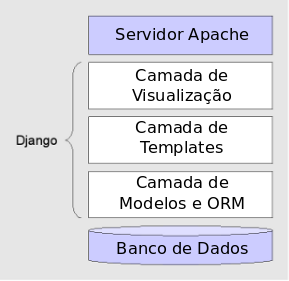
\includegraphics[width=0.9\textwidth]{../Figures/django_layers.png}}
    \caption[Diagrama com a separação entre as camadas do Django]{Nesta figura podemos observar a separação interna do Django entre as camadas de Modelo, de Visualização e de Templates. Fonte:\url{http://excess.org/article/2009/05/django-1-1-talk-text/}}
  \label{fig:django_layers2}
\end{figure}
\end{landscape}
\clearpage
}

A camada de Visualização é responsável por encapsular toda a lógica de processamento de cada requisição que é feita pelo usuário ao Django, é nesta camada onde são aplicados todos os critérios de filtragem de variantes que foram definidos pelos usuário. A camada de Modelo e ORM é responsável pelo acesso ao banco de dados através da criação de consultas em SQL que possuem os critérios de filtragem definidos pelo formulário e finalmente a camada de Templates gera o HTML final com o resultado obtido para o usuário final utilizando HTML, CSS e Javascript. 

\noindent
Site: \url{http://www.djangoproject.org}

\section{Formatos Utilizados}

\subsection{FASTQ}

O formato FASTQ foi proposto pela primeira vez em 2009 por \cite{Cock2009} e surgiu como um formato utilizado para descrever pequenas sequências de DNA chamadas de leituras (\textit{reads}) que são geradas pelos sequenciadores de DNA de nova geração. A característica principal deste formato é o armazenamento em um único arquivo da informação sobre as sequências de DNA que foram lidas e do escore de qualidade de cada base das sequências que estão presentes neste arquivo. 

A figura \ref{fig:fastq_definition} apresenta o exemplo de uma leitura em formato FASTQ. Podemos observar que cada sequência é iniciada pelo simbolo @, seguida de um ID único e com informações como o tamanho de cada leitura que foi lida pela máquina.
O simbolo ``+'' significa indica o início dos valores de qualidade de cada base na próxima linha para a leitura que foi lida anteriormente.

Existem algumas variações deste formato, como por exemplo em sequenciadores do modelo SOLID 5500XL são adicionadas informações sobre valores de qualidade de cada base em \textit{color space}. Esta tecnologia foi criada pela Applied Biosystems e chamada de \textit{2\_base encoding}, de acordo com a empresa, ela permite a leitura de cada base duas vezes sem precisar para isso realizar o sequenciamento dos dados duas vezes.

\afterpage{
\begin{landscape}
\begin{figure}[p]
  \centering
    \Large\textbf{Exemplo de uma leitura em formato FASTQ}\par\medskip   
    \fbox{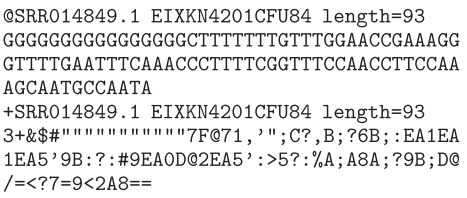
\includegraphics[width=1.5\textwidth]{./Figures/fastq_definition.png}}
    \caption[Exemplo de uma leitura em formato FASTQ]{Nesta figura podemos observar uma leitura que está presente em um arquivo no formato FASTQ. - Fonte: \cite{Cock2009} }
    
  \label{fig:fastq_definition}
\end{figure}
\end{landscape}
\clearpage
}

\subsection{Sequence Alignment Map - Formato SAM}

O formato SAM (Sequence Alignment Map) é um arquivo de texto delimitado por tabulações que foi proposto por Heng Li e Richard Dublin em 2009 \cite{Li2009b} e foi criado para armazenar as informações sobre alinhamentos de sequências como resultado após o mapeamento dessas sequências contra um genoma de referência, como por exemplo, o Genoma Humano.

A figura \ref{fig:sam_file} apresenta o exemplo de um arquivo SAM. O cabeçalho deste arquivo é delimitado pelo símbolo @ no início de cada linha, seguido de uma chave do tipo ID (Ex. HD, SQ, RG) com informações sobre como este arquivo foi gerado e os parâmetros utilizados durante o mapeamento. A segunda parte deste arquivo possui informações sobre todas as regiões mapeadas, contendo os valores de qualidade para cada base do alinhamento e um escore de qualidade médio para toda a região que foi mapeada.

O formato SAM também possui uma versão chamada de BAM, que converte os dados do arquivo SAM para uma linguagem binária (de máquina) ao invés de texto, o que ajuda a reduzir muito o tamanho do arquivo em relação ao seu original, sem que ocorra perda de informação durante essa conversão.

\afterpage{
\begin{landscape}

\begin{figure}[p]
  \centering
    \Large\textbf{Exemplo de um arquivo no formato SAM}\par\medskip   
    \fbox{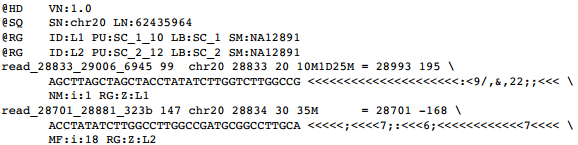
\includegraphics[width=1.5\textwidth]{./Figures/sam_file.png}}
    \caption[Exemplo de um arquivo no formato SAM]{Exemplo de um arquivo no formato SAM proposto por Li. Fonte: \cite{Li2009b}}
  \label{fig:sam_file}
\end{figure}
\end{landscape}

\clearpage
}

\subsection{Variant Call Format - Formato VCF}

O formato VCF (\textit{Variant Call Format}) foi proposto por Danecek em 2011 \cite{Danecek2011} e atualmente está em sua versão 4.2. Ele foi criado para armazenar informações sobre SNPs, Indels e Variantes Estruturais encontrados nos indivíduos sequenciados pelo projeto \textit{1000 Genomes}, juntamente com informações relevantes sobre cada variante de uma maneira compacta e indexada, usando para isso um programa desenvolvido em C chamado tabix \footnote{\url{http://www.htslib.org/doc/tabix.html}}. Este programa permite a recuperação rápida das informações genotípicas de cada indivíduo utilizando posições indexadas em relação a um genoma de referência.

A figura \ref{fig:vcf_format} apresenta um exemplo de um arquivo no formato VCF. Podemos verificar uma separação entre o cabeçalho do arquivo que é sempre iniciado com o símbolo \# e o corpo do arquivo que contém uma linha para cada variante encontrada. Este arquivo permite o armazenamento da informações do genótipo de múltiplos indivíduos, adicionando uma coluna no final do arquivo com a informação sobre o genótipo para cada indivíduo daquela posição. Todos os campos do corpo deste arquivo são separados por tabulações.

\afterpage{
\begin{landscape}

\begin{figure}[p]
  \centering
    \Large\textbf{Exemplo de um arquivo no formato VCF}\par\medskip   
    \fbox{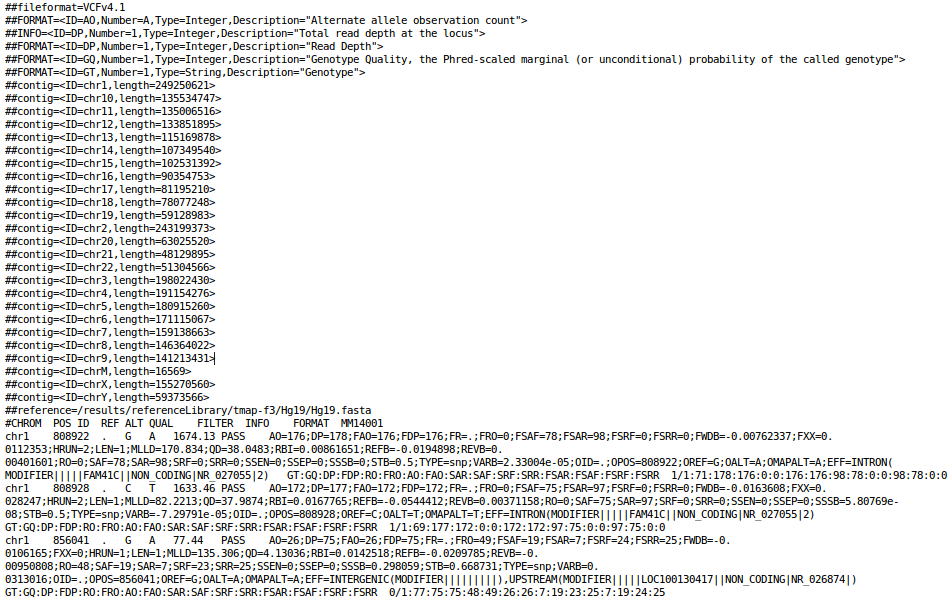
\includegraphics[width=1.2\textwidth]{./Figures/vcf_sample.png}}
    \caption[Exemplo de um arquivo no formato VCF]{Exemplo de um arquivo no formato VCF podemos observar alguns campos do cabeçalho e do corpo.}
  \label{fig:vcf_format}
\end{figure}
\end{landscape}

\clearpage
}

%adicionar o proprio vcf
% \begin{landscape}
% \lstinputlisting{data/clinical_case/vcf_header.vcf}
% \end{landscape}

\section{Programas Utilizados}

\subsection{\textit{FASTQC}}

O \textit{FASTQC} é um programa em Java que oferece uma interface gráfica para análise de dados genômicos em formato FASTQ ou BAM. Este programa permite a geração de relatórios em HTML com imagens que possuem métricas que permitem avaliar a qualidade do sequenciamento.
\noindent
Site: \url{http://www.bioinformatics.babraham.ac.uk/projects/fastqc/}


\subsection{\textit{SAMTOOLS}}

O \textit{SAMTOOLS} é um programa de linha de comando que trabalha com arquivos SAM/BAM e VCF. Além de permitir a indexação e conversão desses arquivos, este programa também possui um algoritmo Bayesiano para identificação de variantes a partir de um arquivo SAM/BAM.

\noindent
Site: \url{http://samtools.sourceforge.net/}


\subsection{\textit{PICARD TOOLS}}

O \textit{PICARD} é um programa em Java criado pelo Broad Intitute que possui ferramentas de linha de comando para a manipulação de arquivos no formato SAM/BAM. Este programa permite ordenar e indexar arquivos SAM/BAM, remover leituras que forem duplicadas, extrair métricas do alinhamento entre muitas outras coisas tarefas.

\noindent
Site: \url{http://picard.sourceforge.net}

\subsection{\textit{Burrows-Wheeler Aligner}}

O programa \textit{BWA} \cite{Li2009a} é um mapeador de leituras desenvolvido por Heng Li e  Richard Durbin que utiliza a transformada de \textit{Burrows-Wheeler} para indexar os genomas e depois realizar o processo de mapeamento das leituras contra um genoma de referência. Este alinhador foi publicado em 2009 e atualmente possui um método chamado \textit{bwa mem} que é o mais utilizado para se alinhar leituras geradas por sequenciadores da empresa Illumina. Este alinhador foi utilizado para o alinhamento do primeiro exoma recebido pelo nosso laboratório.

\noindent
Site: \url{http://bio-bwa.sourceforge.net}

\subsection{\textit{BFAST}}
O \textit{BFAST} \cite{Homer2009} acrônimo de ``BLAT-like Fast Accurate Search Tool'' é um alinhador desenvolvido por Nils Homer da Universidade da Califórnia em Los Angeles. Este programa basicamente realiza o alinhamento das leituras em duas etapas: Primeiro utilizando múltiplos índices de um genoma de referência ele identifica os locais de alinhamento candidatos para cada uma das leituras. Depois ele realiza um alinhamento com GAPs nos locais candidatos que foram identificados no passo anterior para definir aquele que possui a melhor correspondência com cada uma das leituras.

Este programa foi utilizado para a análise dos dados do sequenciador SOLID 5500XL e foi necessário a utilização de um \textit{branch} do \textit{BFAST} chamado de \textit{BFAST}+\textit{BWA} que foi recomendado pelo centro que realizou o sequenciamento dos dados, pois ele utiliza dois algoritmos diferentes para alinhar as leituras \textit{forward} e \textit{reverse} que possuem tamanhos diferentes 75 pb e 35 pb respectivamente.
\noindent
Site: \url{http://bfast.sourceforge.net}

\subsection{\textit{GATK}}

O \textit{Genome Analisys ToolKit} (\textit{GATK}) \cite{DePristo2011}  é um framework desenvolvido em Java pelo Broad Institute que possui diversos métodos utilizados para melhorar a qualidade da análise dos dados além de realizar a identificação das variantes gerando um arquivo VCF no final a partir dos arquivos SAM/BAM do alinhamento. Este programa foi utilizado para a análise de todos os dados recebidos pelo Laboratório de Genômica Clínica e também para realizar a análise dos dados do Projeto 1000Genomes. 

Um diagrama do framework proposto pelo \textit{GATK} para análise dos dados é apresentado na figura \ref{fig:gatk_framework}.

\afterpage{
\begin{landscape}

\begin{figure}[p]
  \centering
    \Large\textbf{GATK Framework de análise de variantes}\par\medskip   
    \fbox{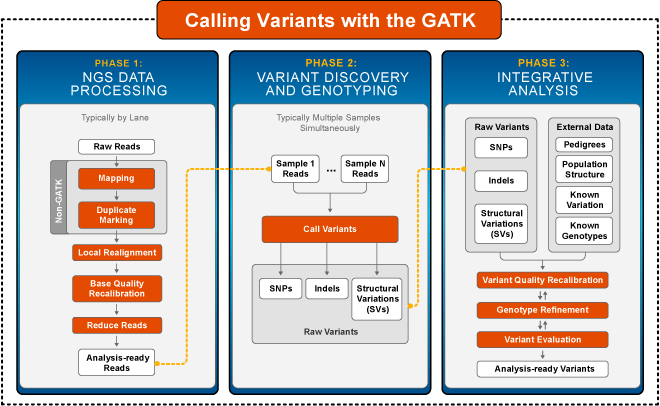
\includegraphics[width=1.4\textwidth]{../Figures/GATK.png}}
    \caption[GATK Framework de análise de variantes]{Nesta figura podemos observar todas as etapas existentes do programa \textit{GATK}. Source: https://www.broadinstitute.org/gatk/ }

  \label{fig:gatk_framework}
\end{figure}
\end{landscape}

\clearpage


}

\noindent
Site: \url{http://www.broadinstitute.org/gatk/}

\subsection{\textit{IGV}}
O \textit{IGV} é um Genome Browser desenvolvido pelo Broad Institute que permite a visualização dos dados genômicos de maneira integrativa permitindo a utilização de arquivos BAM e VCF para visualização de regiões genômicas. Este programa foi utilizado para investigação de algumas variantes candidatas identificadas por diferentes membros do nosso laboratório.
\noindent
Site: \url{http://www.broadinstitute.org/igv/}

\section{Banco de Dados e Programas Utilizadas}

\subsection{1000Genomes}

No site do projeto foi obtido um arquivo com 39.706.715 posições contendo 4 bilhões de genótipos que foram utilizadas como controle no processo de filtragem de variantes baseado em um limiar de frequência dessas variantes calculado sobre 2500 indivíduos.

Site: \url{http://www.1000genomes.org/}

\subsection{Exome Variant Server}

Esse projeto é importante pois já realizou o sequenciamento de mais de 6500 exomas de indivíduos. No site do projeto foi obtido um arquivo VCF com a frequência de 1.872.496 variantes, este arquivo é utilizado durante o processo de anotação de variantes para ajudar a filtrar variantes baseadas na sua frequência.

Site: \url{http://evs.gs.washington.edu/}

\subsection{dbSNP}

O dbSNP é um banco de dados público desenvolvido pelo National Center for Biotechnology Information (NCBI) que armazena informações sobre variações genéticas como SNPs, INDELs que foram encontradas em diferentes espécies como por exemplo: Humanos, Bovinos e Caninos. Os dados de humanos deste banco, atualmente na versão 142, foram utilizados ao longo deste projeto durante a análise dos dados e no processo de filtragem de variantes para ajudar a eliminar variantes comuns, por exemplo,  baseado na frequência dessa variante que foi encontrada em um grupo de indivíduos.

Na tabela \ref{dbsnp137} apresentamos informações sobre o último release do dbSNP versão 137.

\afterpage{
\begin{table}[p]
\captionsetup{font=normalsize}
\caption{Informações sobre o dbSNP 137}
\begin{center}
\begin{tabular}{|l|l|}
\hline
\textbf{Organismo} & Homo sapiens \\ \hline
\textbf{dbSNP Build} & 137 \\ \hline
\textbf{Genome Build} & 37.4 \\ \hline
\textbf{Número de Submissões (ss\#'s)} & 192.678.553 \\ \hline
\textbf{Número de RefSNP Clusters (rs\#'s) ( \# validados)} & 53.567.890 (38.072.522) \\ \hline
\textbf{Número de (rs\#'s) em genes} & 22.450.743 \\ \hline
\textbf{Número de (ss\#'s) com genótipo} & 75.115.460 \\ \hline
\textbf{Número de (ss\#'s) com frequência} & 35.997.781 \\ \hline
\end{tabular}
\end{center}
\label{dbsnp137}
\end{table}
\clearpage
}

Podemos observar que existem atualmente 53,567,890 \textit{reference clustered SNPIDs} (rsids), esses valores são ids únicos atribuídos a cada variante e são utilizados para anotação das frequências de cada variante.

\noindent

Site: \url{http://www.ncbi.nlm.nih.gov/projects/SNP}

\subsection{\textit{GATK Resource Bundle}}
O \textit{GATK Resource Bundle} é um repositório de arquivos recomendados pelo \textit{GATK} para serem utilizados durante a análise de genomas e exomas. Através deste repositório foram obtidos datasets com 292 exomas controles para serem utilizados no processo de filtragem de variantes.
\noindent

Site: \url{http://ftp.broadinstitute.org}

\subsection{\textit{OMIM - Online Mendelian Inheritance in Man}}

O Online Mendelian Inheritance in Man (OMIM) é um banco de dados público de genes associados a doenças Mendelianas. Este banco de dados em julho de 2015 possui 14.965 genes e 5.523  fenótipos associados a doenças Mendelianas. Essas informações foram obtidas e utilizadas para auxiliar na investigação de variantes candidatas. Por exemplo, o usuário pode buscar todos os genes associados a uma doença e visualizar as variantes desses genes presentes em cada um dos indivíduos inseridos no sistema.
\noindent

Site: \url{http://www.omim.org}

\subsection{HGNC - HUGO Gene Nomenclature Committee}

Os dados sobre os genes incluídos no Mendel,MD foram obtidos a partir do site HUGO Gene Nomenclature Committee (HGNC) \cite{Gray2013} que é um banco de dados com ``\textit{gene symbols}'' e nomes únicos para cerca de 37 mil regiões do genoma humano, sendo que mais de 19 mil dessas regiões são consideradas codificadoras de proteínas (genes). 

A tabela \ref{hgnc_genes} apresenta informações sobre os dados que foram obtidos no endereço \url{http://www.genenames.org/cgi-bin/hgnc_stats}. 

\afterpage{
\begin{table}[p]
\caption{Estatísticas sobre os genes de acordo com o HUGO \textit{Gene Nomenclature Committee} (HGNC)}
\begin{center}
\scalebox{1.0}{
\begin{tabular}{|p{1.5cm}|p{3cm}|p{5cm}|p{2cm}|}
\hline
\multicolumn{4}{|c|}{\textbf{Estatísticas sobre o Genome de Referência}} \\ \hline
\textbf{Grupo de Locus} & \textbf{Total por Grupo} & \textbf{Tipo} & \textbf{Total por Tipo de Locus} \\ \hline
\multicolumn{ 1}{|c|}{Gene codificador de proteína} & \multicolumn{ 1}{c|}{19.067} & gene com produto proteico & 19.067 \\ \hline
\multicolumn{ 1}{|c|}{RNA não-codificador} & \multicolumn{ 1}{c|}{4405} & RNA Y & 4 \\ \cline{ 3- 4}
\multicolumn{ 1}{|c|}{} & \multicolumn{ 1}{l|}{} & cluster de RNA  & 125 \\ \cline{ 3- 4}
\multicolumn{ 1}{|c|}{} & \multicolumn{ 1}{l|}{} & RNA longo não codificador & 1690 \\ \cline{ 3- 4}
\multicolumn{ 1}{|c|}{} & \multicolumn{ 1}{l|}{} & microRNA & 1524 \\ \cline{ 3- 4}
\multicolumn{ 1}{|c|}{} & \multicolumn{ 1}{l|}{} & RNA variado & 3 \\ \cline{ 3- 4}
\multicolumn{ 1}{|c|}{} & \multicolumn{ 1}{l|}{} & RNA ribossomal & 34 \\ \cline{ 3- 4}
\multicolumn{ 1}{|c|}{} & \multicolumn{ 1}{l|}{} & RNA pequeno citoplasmático & 3 \\ \cline{ 3- 4}
\multicolumn{ 1}{|c|}{} & \multicolumn{ 1}{l|}{} & RNA pequeno nuclear & 71 \\ \cline{ 3- 4}
\multicolumn{ 1}{|c|}{} & \multicolumn{ 1}{l|}{} & RNA pequeno nucleolar & 414 \\ \cline{ 3- 4}
\multicolumn{ 1}{|c|}{} & \multicolumn{ 1}{l|}{} & RNA de transferência & 533 \\ \cline{ 3- 4}
\multicolumn{ 1}{|c|}{} & \multicolumn{ 1}{l|}{} & RNA cofre & 4 \\ \hline
\multicolumn{ 1}{|c|}{Fenótipos} & \multicolumn{ 1}{c|}{703} & apenas com fenótipos & 703 \\ \hline
\multicolumn{ 1}{|c|}{Pseudogenes} & \multicolumn{ 1}{c|}{11880} & pseudogene receptor de células T & 35 \\ \cline{ 3- 4}
\multicolumn{ 1}{|c|}{} & \multicolumn{ 1}{l|}{} & pseudogene imunoglobulina & 199 \\ \cline{ 3- 4}
\multicolumn{ 1}{|c|}{} & \multicolumn{ 1}{l|}{} & pseudogene & 11.646 \\ \hline
\multicolumn{ 1}{|c|}{Outros} & \multicolumn{ 1}{c|}{1111} & gene do receptor de células T & 207 \\ \cline{ 3- 4}
\multicolumn{ 1}{|c|}{} & \multicolumn{ 1}{l|}{} & constituinte de locus complexo & 27 \\ \cline{ 3- 4}
\multicolumn{ 1}{|c|}{} & \multicolumn{ 1}{l|}{} & retrovírus endógeno & 73 \\ \cline{ 3- 4}
\multicolumn{ 1}{|c|}{} & \multicolumn{ 1}{l|}{} & sítio frágil & 117 \\ \cline{ 3- 4}
\multicolumn{ 1}{|c|}{} & \multicolumn{ 1}{l|}{} & genes de imunoglobulina & 224 \\ \cline{ 3- 4}
\multicolumn{ 1}{|c|}{} & \multicolumn{ 1}{l|}{} & protocaderina & 39 \\ \cline{ 3- 4}
\multicolumn{ 1}{|c|}{} & \multicolumn{ 1}{l|}{} & leitura & 86 \\ \cline{ 3- 4}
\multicolumn{ 1}{|c|}{} & \multicolumn{ 1}{l|}{} & região & 44 \\ \cline{ 3- 4}
\multicolumn{ 1}{|c|}{} & \multicolumn{ 1}{l|}{} & elemento transponível & 4 \\ \cline{ 3- 4}
\multicolumn{ 1}{|c|}{} & \multicolumn{ 1}{l|}{} & desconhecidos & 282 \\ \cline{ 3- 4}
\multicolumn{ 1}{|c|}{} & \multicolumn{ 1}{l|}{} & local de integração de vírus & 8 \\ \hline
\multicolumn{ 3}{|c|}{\textbf{Total de símbolos aprovados}} & 37.166 \\ \hline
\end{tabular}
}
\end{center}
\label{hgnc_genes}
\end{table}
\clearpage
}

Site: \url{http://www.genenames.org}

\subsection{HGMD}

O HGMD \cite{Stenson2009} é um banco de dados comercial com mutações germinativas e nucleares que foram descritas e validadas pela literatura como sendo associadas a doenças humanas. Estes dados foram utilizados para permitir a busca de mutações que já estivessem descritas anteriormente pela literatura.

Site: \url{http://www.hgmd.cf.ac.uk}

\subsection{Genoma Humano de Referência b37}

Todas as análises deste trabalho foram realizadas usando a versão b37 do genoma humano, o mesmo arquivo que foi utilizado pelo projeto 1000genomes para suas análises e está disponível no repositório ``\textit{GATK Resource Bundle}'' no FTP do Broad Institute. Ele seria o equivalente ao hg19 do genoma fornecido pelo UCSC.

A tabela \ref{b37_chrs} apresenta o número de pares de base em cada um dos 84 contigs referentes aos cromossomos além dos contigs que ainda não puderam ser incorporados nos cromossomos. Os contigs iniciados com GL (Genome Library) são sequências que ainda não puderam ser integradas aos contigs canônicos (ex. 1,2,3)
 
\afterpage{
\begin{table}[p]
\caption{Tabela com informações sobre o número de pares de bases de cada um dos cromossomos do genome build b37.}
%     \begin{center}
	\centering
    \begin{tabular}{|l|l|l|l|}
    \hline
    Contig          & Pares de Base & Contig & Pares de Base  \\ \hline
    1          & 249.250.621 & GL000208.1 & 92.689  \\ \hline
    2          & 243.199.373 & GL000209.1 & 159.169 \\ \hline
    3          & 198022.430 & GL000210.1 & 27.682  \\ \hline
    4          & 191.154.276 & GL000211.1 & 166.566 \\ \hline
    5          & 180.915.260 & GL000212.1 & 186.858 \\ \hline
    6          & 171.115.067 & GL000213.1 & 164.239 \\ \hline
    7          & 159.138.663 & GL000214.1 & 137.718 \\ \hline
    8          & 146.364.022 & GL000215.1 & 172.545 \\ \hline
    9          & 141.213.431 & GL000216.1 & 172.294 \\ \hline
    10         & 135.534.747 & GL000217.1 & 172.149 \\ \hline
    11         & 135.006.516 & GL000218.1 & 161.147 \\ \hline
    12         & 133.851.895 & GL000219.1 & 179.198 \\ \hline
    13         & 115.169.878 & GL000220.1 & 161.802 \\ \hline
    14         & 107.349.540 & GL000221.1 & 155.397 \\ \hline
    15         & 102.531.392 & GL000222.1 & 186.861 \\ \hline
    16         & 90.354.753  & GL000223.1 & 180.455 \\ \hline
    17         & 81.195.210  & GL000224.1 & 179.693 \\ \hline
    18         & 78.077.248  & GL000225.1 & 211.173 \\ \hline
    19         & 59.128.983  & GL000226.1 & 15.008  \\ \hline
    20         & 63.025.520  & GL000227.1 & 128.374 \\ \hline
    21         & 48.129.895  & GL000228.1 & 129.120 \\ \hline
    22         & 51.304.566  & GL000229.1 & 19.913  \\ \hline
    X          & 155.270.560 & GL000230.1 & 43.691  \\ \hline
    Y          & 59.373.566  & GL000231.1 & 27.386  \\ \hline
    MT         & 16.569     & GL000232.1 & 40.652  \\ \hline
    GL000191.1 & 106.433    & GL000233.1 & 45.941  \\ \hline
    GL000192.1 & 547.496    & GL000234.1 & 40.531  \\ \hline
    GL000193.1 & 189.789    & GL000235.1 & 34.474  \\ \hline
    GL000194.1 & 191.469    & GL000236.1 & 41.934  \\ \hline
    GL000195.1 & 182.896    & GL000237.1 & 45.867  \\ \hline
    GL000196.1 & 38.914     & GL000238.1 & 39.939  \\ \hline
    GL000197.1 & 37.175     & GL000239.1 & 33.824  \\ \hline
    GL000198.1 & 90.085     & GL000240.1 & 41.933  \\ \hline
    GL000199.1 & 169.874    & GL000241.1 & 42.152  \\ \hline
    GL000200.1 & 187.035    & GL000242.1 & 43.523  \\ \hline
    GL000201.1 & 36.148     & GL000243.1 & 43.341  \\ \hline
    GL000202.1 & 40.103     & GL000244.1 & 39.929  \\ \hline
    GL000203.1 & 37.498     & GL000245.1 & 36.651  \\ \hline
    GL000204.1 & 81.310     & GL000246.1 & 38.154  \\ \hline
    GL000205.1 & 174.588    & GL000247.1 & 36.422  \\ \hline
    GL000206.1 & 41.001     & GL000248.1 & 39.786  \\ \hline
    GL000207.1 & 4.262      & GL000249.1 & 38.502  \\ \hline
    \end{tabular}
% \end{center}

\label{b37_chrs}
\end{table}
\clearpage
}


Site: \url{ftp://ftp-trace.ncbi.nih.gov/1000genomes/ftp/technical/reference/}


\subsection{Escore PHRED}

O escore de qualidade chamado PHRED (Q) é um valor entre 4 e 60 que é dado para cada base de DNA que é lida de acordo com a sua qualidade utilizando uma escala negativa de probabilidade do log dos valores de qualidade. Esse valor é calculado de acordo com a seguinte fórmula:

\[Q=-10\log_{10}P\]

Como exemplo, um phred escore de 10 significa que temos a probabilidade de 1 erro a cada 10 bases, ou seja 90\% de acurácia para cada base que foi lida, já um Phred escore de 60 indica a probabilidade de erro de 1 em 1.000.000 milhão de bases ou seja 99.99999\% de acurácia.

Site: \url{http://www.phrap.com/phred/}

\subsection{Escore SIFT}

O SIFT \cite{Ng2003} é um escore criado para predizer o impacto causado na função da proteína por mudanças na sua sequência de aminoácidos. Esse escore é bastante utilizado para ajudar a identificar boas variantes candidatas. Esse algoritmo utiliza homologia de sequências para predizer se uma substituição do aminoácido pode causar uma mudança na estrutura de uma determinada proteína. Apesar de seu primeiro artigo ter sido publicado em 2001 ainda é bastante utilizado na análise de exomas.

\url{http://sift.jcvi.org/}

\subsection{Escore Polyphen-2}

Esse é um escore de patogenicidade que também é bastante utilizado, porém sua diferença em relação ao SIFT é que quanto maior for o escore mais patogênica tende a ser a variante estudada \cite{Adzhubei2013}. Portanto, valores próximos de 1.0 seriam mais patogênicos de acordo com esse algoritmo.

\url{http://genetics.bwh.harvard.edu/pph2/}

\subsection{Escore CADD}
 
O CADD (\textit{Combined Annotation Dependent Depletion}) é um escore que integra múltiplas anotações em uma única métrica utilizando mutações que sobrevivem a um processo de seleção natural aplicado sobre mutações simuladas ao longo do genoma \cite{Kircher2014a}. Esse escore pode ser utilizado para encontrar mutações patogênicas, porém ao contrário dos escores de SIFT e Polyphen-2, ele não possui valores sugeridos para determinar se uma variante é ou não é patogênica, quanto maior o seu valor maior a chance da variante ser patogênica.

\url{http://cadd.gs.washington.edu/}


\subsection{\textit{SnpEff}}

O \textit{SnpEff} é uma ferramenta para anotação e predição do efeito causado por variantes presentes em diversas regiões de um genoma. Além de realizar a anotação de SNPs e indels que estão localizados nos genes, ele também é capaz de predizer mutações em regiões de \textit{splicing}, regiões com \textit{frameshifts}, perda ou ganho de função entre outras que estão descritas no site da ferramenta.

Na tabela \ref{snpeff_faq} podemos observar que a maioria dos efeitos das variantes que podem causar problemas pertencem as classes HIGH ou MODERATE classificadas por este programa. Estas duas categorias podem ser utilizadas como critério de filtragem durante a análise de exomas para identificação de possíveis genes e mutações candidatas.


\begin{table}[]
\Large 
\centering
\caption{Tabela com as classes de impacto do programa SnpEff}
\label{snpeff_faq}
\scalebox{0.6}{
\begin{tabular}{|l|l|lll}
\cline{1-2}
\textbf{Impacto} & \textbf{Termo Ontológico}                                  &  &  &  \\ \cline{1-2}
HIGH                           & chromosome\_number\_variation                        &  &  &  \\ \cline{1-2}
HIGH                           & exon\_loss\_variant                                  &  &  &  \\ \cline{1-2}
HIGH                           & frameshift\_variant                                  &  &  &  \\ \cline{1-2}
HIGH                           & rare\_amino\_acid\_variant                           &  &  &  \\ \cline{1-2}
HIGH                           & splice\_acceptor\_variant                            &  &  &  \\ \cline{1-2}
HIGH                           & splice\_donor\_variant                               &  &  &  \\ \cline{1-2}
HIGH                           & start\_lost                                          &  &  &  \\ \cline{1-2}
HIGH                           & stop\_gained                                         &  &  &  \\ \cline{1-2}
HIGH                           & stop\_lost                                           &  &  &  \\ \cline{1-2}
HIGH                           & transcript\_ablation                                 &  &  &  \\ \cline{1-2}
MODERATE                       & 3\_prime\_UTR\_truncation +exon\_loss                &  &  &  \\ \cline{1-2}
MODERATE                       & 5\_prime\_UTR\_truncation +exon\_loss\_variant       &  &  &  \\ \cline{1-2}
MODERATE                       & coding\_sequence\_variant                            &  &  &  \\ \cline{1-2}
MODERATE                       & disruptive\_inframe\_deletion                        &  &  &  \\ \cline{1-2}
MODERATE                       & disruptive\_inframe\_insertion                       &  &  &  \\ \cline{1-2}
MODERATE                       & inframe\_deletion                                    &  &  &  \\ \cline{1-2}
MODERATE                       & inframe\_insertion                                   &  &  &  \\ \cline{1-2}
MODERATE                       & missense\_variant                                    &  &  &  \\ \cline{1-2}
MODERATE                       & regulatory\_region\_ablation                         &  &  &  \\ \cline{1-2}
MODERATE                       & splice\_region\_variant                              &  &  &  \\ \cline{1-2}
MODERATE                       & TFBS\_ablation                                       &  &  &  \\ \cline{1-2}
LOW                            & 5\_prime\_UTR\_premature start\_codon\_gain\_variant &  &  &  \\ \cline{1-2}
LOW                            & initiator\_codon\_variant                            &  &  &  \\ \cline{1-2}
LOW                            & splice\_region\_variant                              &  &  &  \\ \cline{1-2}
LOW                            & start\_retained                                      &  &  &  \\ \cline{1-2}
LOW                            & stop\_retained\_variant                              &  &  &  \\ \cline{1-2}
LOW                            & synonymous\_variant                                  &  &  &  \\ \cline{1-2}
MODIFIER                       & 3\_prime\_UTR\_variant                               &  &  &  \\ \cline{1-2}
MODIFIER                       & 5\_prime\_UTR\_variant                               &  &  &  \\ \cline{1-2}
MODIFIER                       & coding\_sequence\_variant                            &  &  &  \\ \cline{1-2}
MODIFIER                       & conserved\_intergenic\_variant                       &  &  &  \\ \cline{1-2}
MODIFIER                       & downstream\_gene\_variant                            &  &  &  \\ \cline{1-2}
MODIFIER                       & conserved\_intron\_variant                           &  &  &  \\ \cline{1-2}
MODIFIER                       & exon\_variant                                        &  &  &  \\ \cline{1-2}
MODIFIER                       & feature\_elongation                                  &  &  &  \\ \cline{1-2}
MODIFIER                       & feature\_truncation                                  &  &  &  \\ \cline{1-2}
MODIFIER                       & gene\_variant                                        &  &  &  \\ \cline{1-2}
MODIFIER                       & intergenic\_region                                   &  &  &  \\ \cline{1-2}
MODIFIER                       & intragenic\_variant                                  &  &  &  \\ \cline{1-2}
MODIFIER                       & intron\_variant                                      &  &  &  \\ \cline{1-2}
MODIFIER                       & mature\_miRNA\_variant                               &  &  &  \\ \cline{1-2}
MODIFIER                       & miRNA                                                &  &  &  \\ \cline{1-2}
MODIFIER                       & NMD\_transcript\_variant                             &  &  &  \\ \cline{1-2}
MODIFIER                       & non\_coding\_transcript\_exon\_variant               &  &  &  \\ \cline{1-2}
MODIFIER                       & non\_coding\_transcript\_variant                     &  &  &  \\ \cline{1-2}
MODIFIER                       & regulatory\_region\_amplification                    &  &  &  \\ \cline{1-2}
MODIFIER                       & regulatory\_region\_variant                          &  &  &  \\ \cline{1-2}
MODIFIER                       & TF\_binding\_site\_variant                           &  &  &  \\ \cline{1-2}
MODIFIER                       & TFBS\_amplification                                  &  &  &  \\ \cline{1-2}
MODIFIER                       & transcript\_amplification                            &  &  &  \\ \cline{1-2}
MODIFIER                       & transcript\_variant                                  &  &  &  \\ \cline{1-2}
MODIFIER                       & upstream\_gene\_variant                              &  &  &  \\ \cline{1-2}
\end{tabular}
}
\end{table}

\noindent
Site: \url{http://snpeff.sourceforge.net}

\subsection{\textit{ANNOVAR}}

O \textit{ANNOVAR} \cite{Wang2010} é um software de anotação genômica que utiliza informações atualizadas de bancos de dados como o 1000Genomes, dbSNP137 e ESP6500 além de ferramentas como SIFT, Polyphen-2, Phylop e Mutation Taster de uma maneira integrada e rápida  para anotar arquivos no formato VCF através de scripts desenvolvidos em Perl.

\noindent
Site: \url{http://www.openbioinformatics.org/annovar}


\subsection{dbNSFP}

O dbNSFP \cite{Liu2011b} é um banco de dados que integra anotações funcionais de diversos algoritmos de predição de variantes e possui cerca de ~75 milhões de SNPs não-sinônimas em sua base de dados. Ele utiliza escores de diferentes ferramentas de predição (Ex. SIFT, Polyphen-2, LRT, MutationTaster e MutationAssessor) e escores de conservação (PhyloP, GERP++ e SiPhy) para o processo de anotação de variantes.

\noindent
Site: \url{http://sites.google.com/site/jpopgen/dbNSFP}

\section{Workflow de Análise de Exomas}

Para análise dos exomas recebidos foi necessário o desenvolvimento de um workflow utilizando os programas: \textit{BWA}, \textit{SAMTOOLS}, \textit{Piccard} e \textit{GATK}.

Este pipeline foi inicialmente desenvolvido em Bash e executado no supercomputador do CENAPAD-MG sendo posteriormente transformado em um script em python para permitir a sua execução no servidor do laboratório, facilitando a integração com os outros scripts desenvolvidos.

A seguir apresentamos um diagrama com o nosso pipeline implementado de acordo com o guia de melhores práticas oferecido pelo site do \textit{GATK} no endereço: \url{http://www.broadinstitute.org/gatk/guide/article?id=15}

Na figura \ref{fig:exome_pipeline} podemos visualizar um diagrama com todas as etapas e os processos utilizados neste pipeline:

\afterpage{
\begin{landscape}

\begin{figure}[p]
  \centering
    \Large\textbf{Diagrama com o pipeline de análise de exomas}\par\medskip   
    \fbox{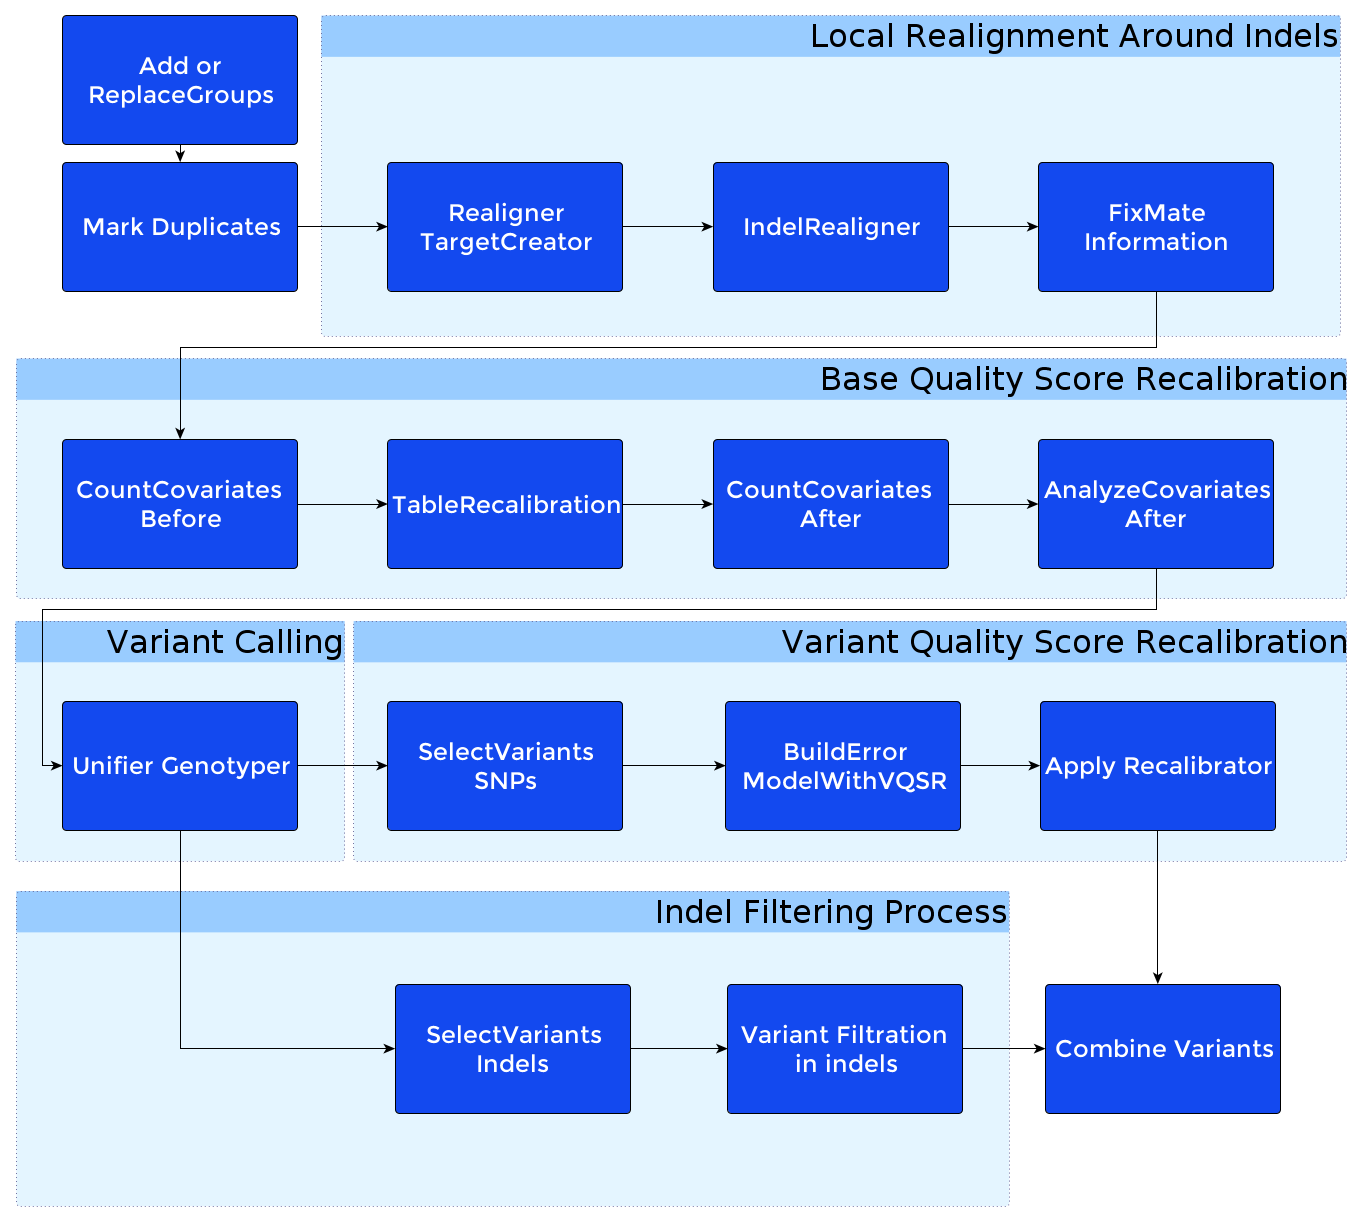
\includegraphics[width=0.9\textwidth]{../Diagramas/gatk_pipelinev2.png}}
    \caption[Diagrama com o pipeline de análise de exomas]{Pipeline desenvolvido para realizar a análise de exomas utilizando o \textit{GATK}. Nesta figura é possivel observar que existem subetapas dentro de cada etapa proposta pelo GATK.}
    
  \label{fig:exome_pipeline}
\end{figure}
\end{landscape}

\clearpage
}

Além do \textit{GATK} outros programas que aceitam arquivos BAMs como entrada foram utilizados para identificação de CNVs e  Short Tandem Repeats (STRs) \cite{Gymrek2012,Krumm2012a,Li2012}.

\subsection{Alinhamento dos dados de SOLID 5500xl}

Para dos dados do sequenciador SOLID 5500xl foi necessário o desenvolvimento de um novo pipeline utilizando uma versão modificada do alinhador \textit{BFAST} que possui uma implementação do \textit{BWA} para alinhar leituras curtas. As leituras deste sequenciador possuem tamanhos diferentes sendo 75 pb para a sequência forward e 35 pb para a sequência reverse, portanto cada uma precisa ser alinhada com um algoritmo diferente. Este alinhador foi recomendado pelo Sick Children Hospital de Toronto que é o lugar onde os dados foram gerados.

